% Options for packages loaded elsewhere
\PassOptionsToPackage{unicode}{hyperref}
\PassOptionsToPackage{hyphens}{url}
\PassOptionsToPackage{dvipsnames,svgnames*,x11names*}{xcolor}
%
\documentclass[
  10pt,
]{krantz}
\usepackage{amsmath,amssymb}
\usepackage{lmodern}
\usepackage{ifxetex,ifluatex}
\ifnum 0\ifxetex 1\fi\ifluatex 1\fi=0 % if pdftex
  \usepackage[T1]{fontenc}
  \usepackage[utf8]{inputenc}
  \usepackage{textcomp} % provide euro and other symbols
\else % if luatex or xetex
  \usepackage{unicode-math}
  \defaultfontfeatures{Scale=MatchLowercase}
  \defaultfontfeatures[\rmfamily]{Ligatures=TeX,Scale=1}
  \setmonofont[Scale=0.7]{Source Code Pro}
\fi
% Use upquote if available, for straight quotes in verbatim environments
\IfFileExists{upquote.sty}{\usepackage{upquote}}{}
\IfFileExists{microtype.sty}{% use microtype if available
  \usepackage[]{microtype}
  \UseMicrotypeSet[protrusion]{basicmath} % disable protrusion for tt fonts
}{}
\makeatletter
\@ifundefined{KOMAClassName}{% if non-KOMA class
  \IfFileExists{parskip.sty}{%
    \usepackage{parskip}
  }{% else
    \setlength{\parindent}{0pt}
    \setlength{\parskip}{6pt plus 2pt minus 1pt}}
}{% if KOMA class
  \KOMAoptions{parskip=half}}
\makeatother
\usepackage{xcolor}
\IfFileExists{xurl.sty}{\usepackage{xurl}}{} % add URL line breaks if available
\IfFileExists{bookmark.sty}{\usepackage{bookmark}}{\usepackage{hyperref}}
\hypersetup{
  pdftitle={Elementos de la estadística},
  pdfauthor={Ricardo Michel MALLQUI BAÑOS},
  colorlinks=true,
  linkcolor=Maroon,
  filecolor=Maroon,
  citecolor=Blue,
  urlcolor=Blue,
  pdfcreator={LaTeX via pandoc}}
\urlstyle{same} % disable monospaced font for URLs
\usepackage{color}
\usepackage{fancyvrb}
\newcommand{\VerbBar}{|}
\newcommand{\VERB}{\Verb[commandchars=\\\{\}]}
\DefineVerbatimEnvironment{Highlighting}{Verbatim}{commandchars=\\\{\}}
% Add ',fontsize=\small' for more characters per line
\usepackage{framed}
\definecolor{shadecolor}{RGB}{248,248,248}
\newenvironment{Shaded}{\begin{snugshade}}{\end{snugshade}}
\newcommand{\AlertTok}[1]{\textcolor[rgb]{0.94,0.16,0.16}{#1}}
\newcommand{\AnnotationTok}[1]{\textcolor[rgb]{0.56,0.35,0.01}{\textbf{\textit{#1}}}}
\newcommand{\AttributeTok}[1]{\textcolor[rgb]{0.77,0.63,0.00}{#1}}
\newcommand{\BaseNTok}[1]{\textcolor[rgb]{0.00,0.00,0.81}{#1}}
\newcommand{\BuiltInTok}[1]{#1}
\newcommand{\CharTok}[1]{\textcolor[rgb]{0.31,0.60,0.02}{#1}}
\newcommand{\CommentTok}[1]{\textcolor[rgb]{0.56,0.35,0.01}{\textit{#1}}}
\newcommand{\CommentVarTok}[1]{\textcolor[rgb]{0.56,0.35,0.01}{\textbf{\textit{#1}}}}
\newcommand{\ConstantTok}[1]{\textcolor[rgb]{0.00,0.00,0.00}{#1}}
\newcommand{\ControlFlowTok}[1]{\textcolor[rgb]{0.13,0.29,0.53}{\textbf{#1}}}
\newcommand{\DataTypeTok}[1]{\textcolor[rgb]{0.13,0.29,0.53}{#1}}
\newcommand{\DecValTok}[1]{\textcolor[rgb]{0.00,0.00,0.81}{#1}}
\newcommand{\DocumentationTok}[1]{\textcolor[rgb]{0.56,0.35,0.01}{\textbf{\textit{#1}}}}
\newcommand{\ErrorTok}[1]{\textcolor[rgb]{0.64,0.00,0.00}{\textbf{#1}}}
\newcommand{\ExtensionTok}[1]{#1}
\newcommand{\FloatTok}[1]{\textcolor[rgb]{0.00,0.00,0.81}{#1}}
\newcommand{\FunctionTok}[1]{\textcolor[rgb]{0.00,0.00,0.00}{#1}}
\newcommand{\ImportTok}[1]{#1}
\newcommand{\InformationTok}[1]{\textcolor[rgb]{0.56,0.35,0.01}{\textbf{\textit{#1}}}}
\newcommand{\KeywordTok}[1]{\textcolor[rgb]{0.13,0.29,0.53}{\textbf{#1}}}
\newcommand{\NormalTok}[1]{#1}
\newcommand{\OperatorTok}[1]{\textcolor[rgb]{0.81,0.36,0.00}{\textbf{#1}}}
\newcommand{\OtherTok}[1]{\textcolor[rgb]{0.56,0.35,0.01}{#1}}
\newcommand{\PreprocessorTok}[1]{\textcolor[rgb]{0.56,0.35,0.01}{\textit{#1}}}
\newcommand{\RegionMarkerTok}[1]{#1}
\newcommand{\SpecialCharTok}[1]{\textcolor[rgb]{0.00,0.00,0.00}{#1}}
\newcommand{\SpecialStringTok}[1]{\textcolor[rgb]{0.31,0.60,0.02}{#1}}
\newcommand{\StringTok}[1]{\textcolor[rgb]{0.31,0.60,0.02}{#1}}
\newcommand{\VariableTok}[1]{\textcolor[rgb]{0.00,0.00,0.00}{#1}}
\newcommand{\VerbatimStringTok}[1]{\textcolor[rgb]{0.31,0.60,0.02}{#1}}
\newcommand{\WarningTok}[1]{\textcolor[rgb]{0.56,0.35,0.01}{\textbf{\textit{#1}}}}
\usepackage{longtable,booktabs,array}
\usepackage{calc} % for calculating minipage widths
% Correct order of tables after \paragraph or \subparagraph
\usepackage{etoolbox}
\makeatletter
\patchcmd\longtable{\par}{\if@noskipsec\mbox{}\fi\par}{}{}
\makeatother
% Allow footnotes in longtable head/foot
\IfFileExists{footnotehyper.sty}{\usepackage{footnotehyper}}{\usepackage{footnote}}
\makesavenoteenv{longtable}
\usepackage{graphicx}
\makeatletter
\def\maxwidth{\ifdim\Gin@nat@width>\linewidth\linewidth\else\Gin@nat@width\fi}
\def\maxheight{\ifdim\Gin@nat@height>\textheight\textheight\else\Gin@nat@height\fi}
\makeatother
% Scale images if necessary, so that they will not overflow the page
% margins by default, and it is still possible to overwrite the defaults
% using explicit options in \includegraphics[width, height, ...]{}
\setkeys{Gin}{width=\maxwidth,height=\maxheight,keepaspectratio}
% Set default figure placement to htbp
\makeatletter
\def\fps@figure{htbp}
\makeatother
\setlength{\emergencystretch}{3em} % prevent overfull lines
\providecommand{\tightlist}{%
  \setlength{\itemsep}{0pt}\setlength{\parskip}{0pt}}
\setcounter{secnumdepth}{5}
\usepackage[spanish,es-lcroman,es-tabla]{babel}
\usepackage{booktabs}
\usepackage{graphicx} 
\usepackage{amsmath}
\usepackage{makeidx}
\usepackage{array}% http://ctan.org/pkg/array
\makeindex


\makeatletter\@addtoreset{chapter}{part}\makeatother%

%\usepackage{showframe}
%\usepackage[a4paper]{geometry}
%\geometry{verbose,tmargin=3cm,bmargin=3cm,lmargin=3.5cm,rmargin=3cm}
\setlength{\tabcolsep}{0.38em}
%\renewcommand{\arraystretch}{1.5}

\usepackage{times}
\renewcommand{\rmdefault}{ptm}
%\usepackage[lite,subscriptcorrection,nofontinfo,zswash]{mtpro2}

\usepackage{graphicx}

% Determine if the image is too wide for the page.
\makeatletter
\def\ScaleIfNeeded{%
  \ifdim\Gin@nat@width>\linewidth
    \linewidth
  \else
    \Gin@nat@width
  \fi
}
\makeatother

% Resize figures that are too wide for the page.
\let\oldincludegraphics\includegraphics
\renewcommand\includegraphics[2][]{%
  \oldincludegraphics[scale=0.85]{#2}
}

\usepackage{amsthm}
\makeatletter
\def\thm@space@setup{%
  \thm@preskip=8pt plus 2pt minus 4pt
  \thm@postskip=\thm@preskip
}
\makeatother



%\flushbottom 

\frontmatter

\ifluatex
  \usepackage{selnolig}  % disable illegal ligatures
\fi
\usepackage[]{natbib}
\bibliographystyle{apalike}

\title{Elementos de la estadística}
\usepackage{etoolbox}
\makeatletter
\providecommand{\subtitle}[1]{% add subtitle to \maketitle
  \apptocmd{\@title}{\par {\large #1 \par}}{}{}
}
\makeatother
\subtitle{estadística descriptiva y probabilidades}
\author{Ricardo Michel MALLQUI BAÑOS}
\date{2021-10-06}

\usepackage{amsthm}
\newtheorem{theorem}{Teorema}[chapter]
\newtheorem{lemma}{Lema}[chapter]
\newtheorem{corollary}{Corolario}[chapter]
\newtheorem{proposition}{Proposición}[chapter]
\newtheorem{conjecture}{Conjectura}[chapter]
\theoremstyle{definition}
\newtheorem{definition}{Definición}[chapter]
\theoremstyle{definition}
\newtheorem{example}{Ejemplo}[chapter]
\theoremstyle{definition}
\newtheorem{exercise}{Ejercicio}[chapter]
\theoremstyle{definition}
\newtheorem{hypothesis}{Hypothesis}[chapter]
\theoremstyle{remark}
\newtheorem*{remark}{Observación}
\newtheorem*{solution}{Solución}
\begin{document}
\maketitle

%\cleardoublepage\newpage\thispagestyle{empty}\null
%\cleardoublepage\newpage\thispagestyle{empty}\null
%\cleardoublepage\newpage
\thispagestyle{empty}
\begin{center}

\includegraphics{U.pdf}
\end{center}

%\setlength{\abovedisplayskip}{-5pt}
%\setlength{\abovedisplayshortskip}{-5pt}

{
\hypersetup{linkcolor=}
\setcounter{tocdepth}{2}
\tableofcontents
}
\listoftables
\listoffigures
\newcommand{\N}{\mathbb{N}}
\newcommand{\R}{\mathbb{R}}
\newcommand{\CC}{\mathbb{C}}
\newcommand{\I}{\mathbb{I}}
\newcommand{\f}{\mathbb{f}}
\newcommand{\X}{\mathbb{X}}
\newcommand{\D}{\mathbb{D}}
\newcommand{\Z}{\mathbb{Z}}
\newcommand{\Q}{\mathbb{Q}}
\newcommand{\norm}[1]{\left\Vert#1\right\Vert}
\newcommand{\abs}[1]{\left\vert#1\right\vert}
\newcommand{\set}[1]{\left\{#1\right\}}
\newcommand{\seq}[1]{\left<#1\right>}
\newcommand{\co}[1]{\left[#1\right]}
\newcommand{\cc}[1]{\left(#1\right)}
\newcommand{\J}{\mathcal{J}}
\newcommand{\K}{\mathcal{K}}
\newcommand{\M}{\mathcal{M}}
\newcommand{\F}{\mathcal{F}}

\hypertarget{resumen}{%
\chapter*{Resumen}\label{resumen}}


La estadística es la ciencia que manipula datos las analiza e interpreta para poder sacar concluciones razonables de ciertos fenomenos naturales. Esta ciencia puede ser dividido en dos: \textbf{estadística descirptiva} y \textbf{estadística inferencial}. En la estadística descriptiva se procesan datos de una manera teórica y utilitaria. Estos métodos consisten en la recolección, organización, resumen, descripcion y presenatacion de la información. Si la poblacion está disponible entonces la estadística descriptiva es suficiente para describir ciertos fenomenos. No obstante generalmente no se dispone de toda la población si no de una muestra de ella, es en este caso que se requieren usar técnicas más sofisticadas para tomar decisiones y generalizaciones acerca de la poblacion, desde una pequeña muestra de información. Es cuando entra en el juego la estadística inferencial.

La base teórica de la estadística son las matemáticas

Este libro se compone de dos partes, la primera parte trata sobre la \textbf{estadística descirptiva} y la segunda \textbf{estadística inferencial}. Cada una de ellas divididas en capítulos.

\mainmatter

\hypertarget{part-estaduxedstica-descriptiva}{%
\part{Estadística descriptiva}\label{part-estaduxedstica-descriptiva}}

\hypertarget{prerrequisitos}{%
\chapter{Prerrequisitos}\label{prerrequisitos}}

WWWWWWWWWWWWWWWWWWWWWWWWWWWWWWWWWWWW

\hypertarget{medidas-de-asimetria}{%
\chapter{Medidas de asimetria}\label{medidas-de-asimetria}}

\hypertarget{datos-no-agrupados}{%
\subsection{Datos no agrupados}\label{datos-no-agrupados}}

Si \[P_k=\frac{k(n+1)}{100}; k=1, 2,  \ldots, 99\] es entero entonces el cuartil es el dato de la posicion \(P_k=x_\frac{k(n+1)}{100}\)
Si \[P_k=\frac{k(n+1)}{100}\] no es entero entonces el cuartil es la interpolacion lineal de de los dos valores entre las cuales se encuentra \(Q_k=\frac{k(n+1)}{100}\)

\begin{itemize}
\tightlist
\item
  Ejemplo
  1, 2, 5, 1 ,5, 6, 7, 8, 9, 3, 4, 5, 2, 6, 2, 5, 6, 7
  Al ordenar de manera creciente
  1, 2, 5, 1 ,5, 6, 7, 8, 9, 3, 4, 5, 2, 6, 2, 5, 6, 7
  y
  \[P_k=\frac{k(18+1)}{100}\]
\end{itemize}

\hypertarget{datos-agrupados}{%
\subsection{Datos agrupados}\label{datos-agrupados}}

\[P_k=L_i+ A\left(\frac{\frac{kn}{100}-F_{i-1}}{F_i-F_{i-1}}\right)=\int_1^3f(x)\]

\begin{longtable}[]{@{}cccc@{}}
\toprule
Clase & \(Y_i\) & \(f_i\) & \(F_i\) \\
\midrule
\endhead
\([5,10)\) & 7.5 & 1 & 1 \\
\([10,15)\) & 12.5 & 2 & 3 \\
\([15,20)\) & 17.5 & 5 & \\
\([20,25)\) & 22.5 & 7 & \\
\([25,30]\) & & 10 & \\
\([30,35]\) & & 6 & \\
\([35,40]\) & & 5 & \\
\([40,45]\) & & 3 & \\
\(\sum\) & & 2 & \\
\bottomrule
\end{longtable}

\hypertarget{datos-no-agrupados-1}{%
\subsection{Datos no agrupados}\label{datos-no-agrupados-1}}

Si \[P_k=\frac{k(n+1)}{100}; k=1, 2,  \ldots, 99\] es entero entonces el cuartil es el dato de la posicion \(P_k=x_\frac{k(n+1)}{100}\)
Si \[P_k=\frac{k(n+1)}{100}\] no es entero entonces el cuartil es la interpolacion lineal de de los dos valores entre las cuales se encuentra \(Q_k=\frac{k(n+1)}{100}\)

\begin{itemize}
\tightlist
\item
  Ejemplo
  1, 2, 5, 1 ,5, 6, 7, 8, 9, 3, 4, 5, 2, 6, 2, 5, 6, 7
  Al ordenar de manera creciente
  1, 2, 5, 1 ,5, 6, 7, 8, 9, 3, 4, 5, 2, 6, 2, 5, 6, 7
  y
  \[P_k=\frac{k(18+1)}{100}\]
\end{itemize}

\hypertarget{datos-agrupados-1}{%
\subsection{Datos agrupados}\label{datos-agrupados-1}}

\[P_k=L_i+ A\left(\frac{\frac{kn}{100}-F_{i-1}}{F_i-F_{i-1}}\right)=\int_1^3f(x)\]

\begin{longtable}[]{@{}cccc@{}}
\toprule
Clase & \(Y_i\) & \(f_i\) & \(F_i\) \\
\midrule
\endhead
\([5,10)\) & 7.5 & 1 & 1 \\
\([10,15)\) & 12.5 & 2 & 3 \\
\([15,20)\) & 17.5 & 5 & \\
\([20,25)\) & 22.5 & 7 & \\
\([25,30]\) & & 10 & \\
\([30,35]\) & & 6 & \\
\([35,40]\) & & 5 & \\
\([40,45]\) & & 3 & \\
\(\sum\) & & 2 & \\
\bottomrule
\end{longtable}

\hypertarget{wwwwww}{%
\section{wwwwww}\label{wwwwww}}

\hypertarget{datos-no-agrupados-2}{%
\subsection{Datos no agrupados}\label{datos-no-agrupados-2}}

Si \[P_k=\frac{k(n+1)}{100}; k=1, 2,  \ldots, 99\] es entero entonces el cuartil es el dato de la posicion \(P_k=x_\frac{k(n+1)}{100}\)
Si \[P_k=\frac{k(n+1)}{100}\] no es entero entonces el cuartil es la interpolacion lineal de de los dos valores entre las cuales se encuentra \(Q_k=\frac{k(n+1)}{100}\)

\begin{itemize}
\tightlist
\item
  Ejemplo
  1, 2, 5, 1 ,5, 6, 7, 8, 9, 3, 4, 5, 2, 6, 2, 5, 6, 7
  Al ordenar de manera creciente
  1, 2, 5, 1 ,5, 6, 7, 8, 9, 3, 4, 5, 2, 6, 2, 5, 6, 7
  y
  \[P_k=\frac{k(18+1)}{100}\]
\end{itemize}

\hypertarget{datos-agrupados-2}{%
\subsection{Datos agrupados}\label{datos-agrupados-2}}

\[P_k=L_i+ A\left(\frac{\frac{kn}{100}-F_{i-1}}{F_i-F_{i-1}}\right)=\int_1^3f(x)=\int_1^3\]

\begin{longtable}[]{@{}cccc@{}}
\toprule
Clase & \(Y_i\) & \(f_i\) & \(F_i\) \\
\midrule
\endhead
\([5,10)\) & 7.5 & 1 & 1 \\
\([10,15)\) & 12.5 & 2 & 3 \\
\([15,20)\) & 17.5 & 5 & \\
\([20,25)\) & 22.5 & 7 & \\
\([25,30]\) & & 10 & \\
\([30,35]\) & & 6 & \\
\([35,40]\) & & 5 & \\
\([40,45]\) & & 3 & \\
\(\sum\) & & 2 & \\
\bottomrule
\end{longtable}

\hypertarget{medidas-de-curtosis-o-apuntamiento}{%
\chapter{Medidas de curtosis o apuntamiento}\label{medidas-de-curtosis-o-apuntamiento}}

En estadística, usamos la medida de curtosis para describir la ``cola'' de la distribución, ya que describe la forma de la misma. También es una medida del ``pico'' de la distribución. Una distribución de curtosis alta tiene un pico más agudo y colas más largas y gruesas, mientras que una distribución de curtosis baja tiene un maní más redondeado y colas más cortas y delgadas.

Datos no agrupados
\[k= \frac{\sum_{i=1}^{n}\left( x_i-\overline{x} \right)^4 }{n} \]

Datos agrupados
\[ K=\frac{\sum_{i=1}^{n}\left( x_i-\overline{x} \right)^4 }{n} \]

\begin{itemize}
\tightlist
\item
  \textbf{Mesocurtico} : esta es la distribución normal
\item
  \textbf{Leptocurtica} : esta distribución tiene colas más gruesas y un pico más afilado. La curtosis es ``positiva'' con un valor superior a 3
\item
  \textbf{Platicurtica} : La distribución tiene un pico más bajo y más ancho y colas más delgadas. La curtosis es ``negativa'' con un valor superior a 3
\end{itemize}

\begin{figure}
\centering
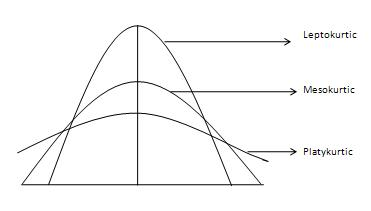
\includegraphics{curtosis.jpg}
\caption{\url{https://link}}
\end{figure}

\hypertarget{medidas-de-asimetruxeda}{%
\chapter{Medidas de asimetría}\label{medidas-de-asimetruxeda}}

Podemos decir que la asimetría indica cuánto se desvía nuestra distribución subyacente de la distribución normal, ya que la distribución normal tiene asimetría 0. Generalmente, tenemos tres tipos de asimetría.

\begin{itemize}
\tightlist
\item
  \textbf{Simétrico} : cuando la asimetría es cercana a 0 y la media es casi la misma que la mediana
\item
  \textbf{Desviación negativa} : cuando la cola izquierda del histograma de la distribución es más larga y la mayoría de las observaciones se concentran en la cola derecha. En este caso, también podemos utilizar el término ``sesgado a la izquierda'' o ``cola izquierda''. y la mediana es mayor que la media.
\item
  \textbf{Desviación positiva} : cuando la cola derecha del histograma de la distribución es más larga y la mayoría de las observaciones se concentran en la cola izquierda. En este caso, también podemos usar el término ``sesgado a la derecha'' o ``cola derecha''. y la mediana es menor que la media.
\end{itemize}

\begin{figure}
\centering
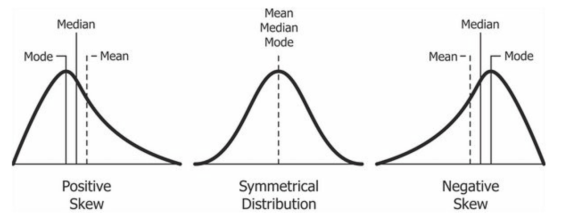
\includegraphics{simetria.png}
\caption{alt}
\end{figure}

\begin{Shaded}
\begin{Highlighting}[]
\NormalTok{data }\OtherTok{=} \FunctionTok{c}\NormalTok{(}\DecValTok{88}\NormalTok{, }\DecValTok{95}\NormalTok{, }\DecValTok{92}\NormalTok{, }\DecValTok{97}\NormalTok{, }\DecValTok{96}\NormalTok{, }\DecValTok{97}\NormalTok{, }\DecValTok{94}\NormalTok{, }\DecValTok{86}\NormalTok{, }\DecValTok{91}\NormalTok{, }\DecValTok{95}\NormalTok{, }\DecValTok{97}\NormalTok{, }\DecValTok{88}\NormalTok{, }\DecValTok{85}\NormalTok{, }\DecValTok{76}\NormalTok{, }\DecValTok{68}\NormalTok{)}
\FunctionTok{hist}\NormalTok{(data, }\AttributeTok{col=}\StringTok{\textquotesingle{}steelblue\textquotesingle{}}\NormalTok{)}
\end{Highlighting}
\end{Shaded}

\begin{center}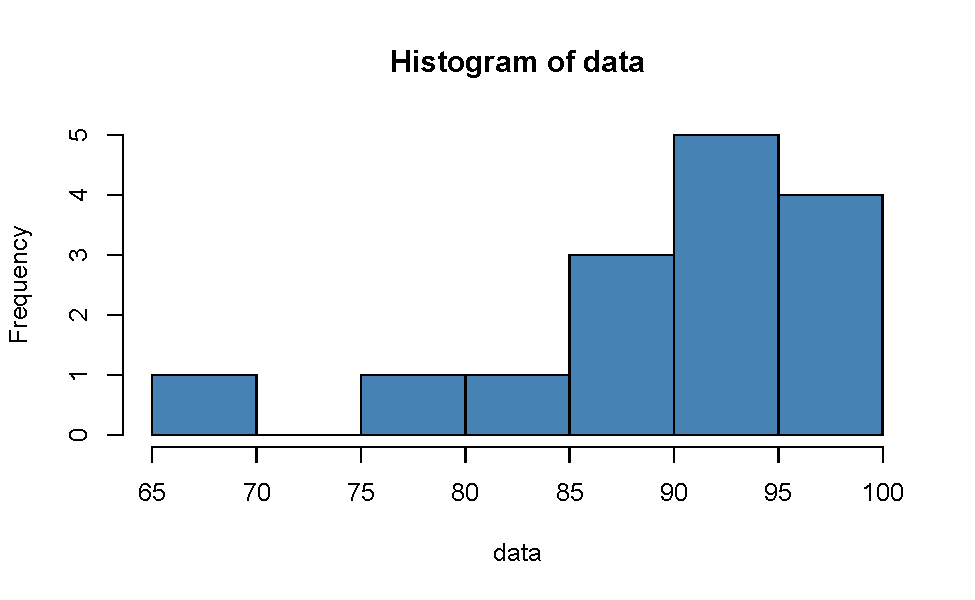
\includegraphics{E_1_files/figure-latex/unnamed-chunk-14-1} \end{center}

\begin{Shaded}
\begin{Highlighting}[]
\NormalTok{dens }\OtherTok{\textless{}{-}} \FunctionTok{density}\NormalTok{(data)}
\FunctionTok{plot}\NormalTok{(dens, }\AttributeTok{frame =} \ConstantTok{FALSE}\NormalTok{, }\AttributeTok{col =} \StringTok{"steelblue"}\NormalTok{, }
     \AttributeTok{main =} \StringTok{"Density plot of mpg"}\NormalTok{) }
\FunctionTok{polygon}\NormalTok{(dens, }\AttributeTok{col =} \StringTok{"steelblue"}\NormalTok{)}
\end{Highlighting}
\end{Shaded}

\begin{center}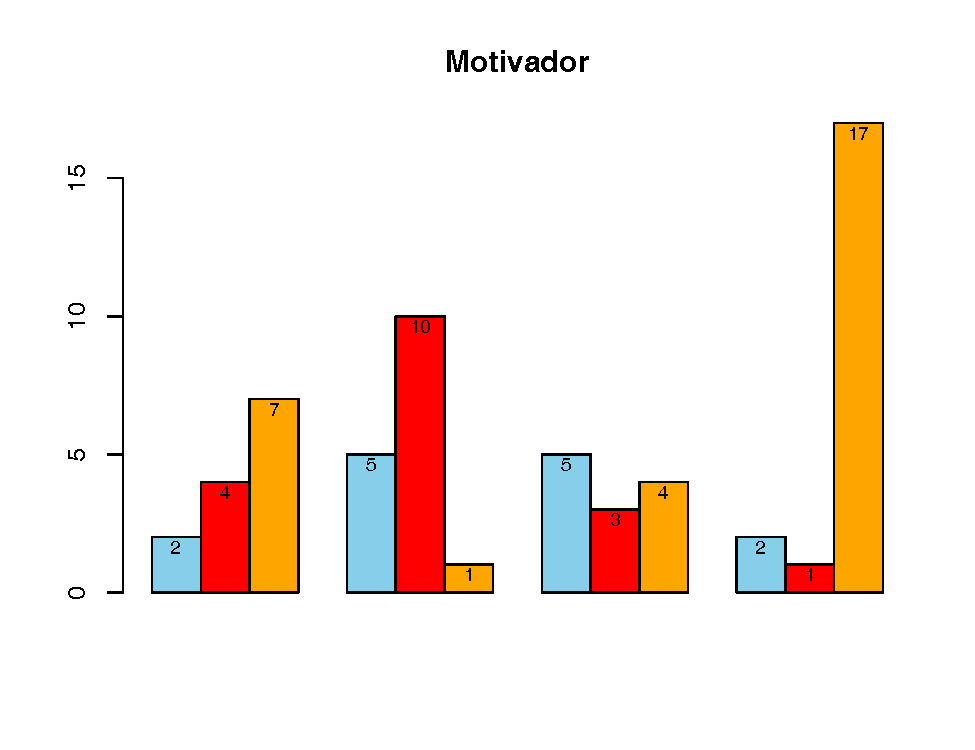
\includegraphics{E_1_files/figure-latex/unnamed-chunk-14-2} \end{center}

\begin{Shaded}
\begin{Highlighting}[]
\FunctionTok{ggplot}\NormalTok{(}\AttributeTok{data=}\NormalTok{iris, }\FunctionTok{aes}\NormalTok{(Petal.Length,}\AttributeTok{fill=}\NormalTok{Species)) }\SpecialCharTok{+}
\FunctionTok{geom\_density}\NormalTok{(}\AttributeTok{alpha=}\FloatTok{0.7}\NormalTok{) }\CommentTok{\# dibujamos el diagrama de densidad}
\end{Highlighting}
\end{Shaded}

\begin{center}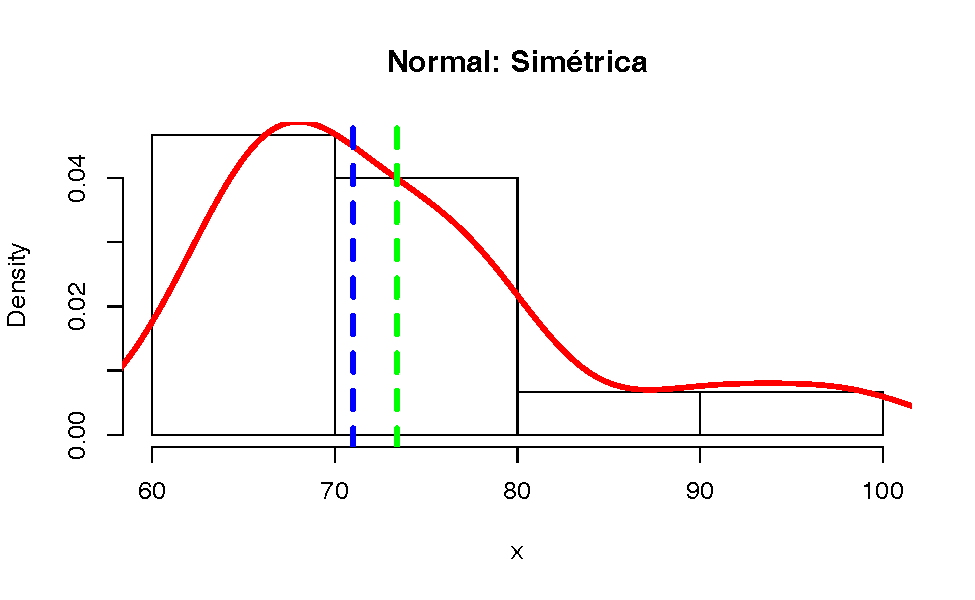
\includegraphics{E_1_files/figure-latex/unnamed-chunk-15-1} \end{center}

\hypertarget{part-probabilidades}{%
\part{Probabilidades}\label{part-probabilidades}}

\hypertarget{experimento-aleatorio}{%
\chapter{Experimento aleatorio}\label{experimento-aleatorio}}

\begin{definition}[Experimento aleatorio]
\protect\hypertarget{def:unnamed-chunk-16}{}{\label{def:unnamed-chunk-16} \iffalse (Experimento aleatorio) \fi{} }En experiento aleatorio es un fenomeno que genera un evento
\end{definition}

\hypertarget{uxe1lgebra-de-eventos}{%
\chapter{Álgebra de eventos}\label{uxe1lgebra-de-eventos}}

Sean \(A\), \(B\) y \(C\) eventos entonces
1. e
2. wwwwwwwwwwwwwwwwwwwwwwwwwwwwww

\[ \int_{1}^{2}=\sum_{2}^{2}x_1 \]

\hypertarget{tuxe9cnicas-de-conteo}{%
\chapter{Técnicas de conteo}\label{tuxe9cnicas-de-conteo}}

\(P_n^m\)
\(C_n^m\)

\[\binom{m}{n}=\frac{m}{n!(n-m)}\]

\hypertarget{definiciuxf3n-de-probabilidad}{%
\chapter{Definición de probabilidad}\label{definiciuxf3n-de-probabilidad}}

\hypertarget{probabilidad-condicional}{%
\chapter{Probabilidad condicional}\label{probabilidad-condicional}}

\[P(A|B)= \frac{P(B\cap A)}{P(B)}\]

\hypertarget{teorema-de-bayes}{%
\chapter{Teorema de Bayes}\label{teorema-de-bayes}}

\begin{theorem}[Teorema de Bayes]
\protect\hypertarget{thm:unnamed-chunk-17}{}{\label{thm:unnamed-chunk-17} \iffalse (Teorema de Bayes) \fi{} }Sea \(\{A_{1},A_{2},...,A_{i},...,A_{n}\}\) un conjunto de sucesos mutuamente excluyentes y exhaustivos, y tales que la probabilidad de cada uno de ellos es distinta de cero (0). Sea \(B\) un suceso cualquiera del que se conocen las probabilidades condicionales \(P(B|A_i )\). Entonces, la probabilidad \(P(A_i|B)\) viene dada por la expresión:
\[P(A_i|B)=\frac{P(B|A_i)P(A_i)}{P(B)}\]
donde:

\begin{enumerate}
\def\labelenumi{\arabic{enumi}.}
\tightlist
\item
  \(P(A_i)\) son las probabilidades a priori,
\item
  \(P(B|A_i)\) es la probabilidad de B en la hipótesis \(A_i\),
\item
  \(P(A_i|B)\) son las probabilidades a posteriori.
\end{enumerate}
\end{theorem}

\hypertarget{eventos-independientes-y-secuencias-de-experimentos}{%
\chapter{Eventos independientes y secuencias de experimentos}\label{eventos-independientes-y-secuencias-de-experimentos}}

\hypertarget{probabilidad-en-espacio}{%
\chapter{Probabilidad en espacio}\label{probabilidad-en-espacio}}

\hypertarget{part-inferencia-estaduxedstica}{%
\part{Inferencia estadística}\label{part-inferencia-estaduxedstica}}

\hypertarget{variables-aleatorias}{%
\chapter{Variables aleatorias}\label{variables-aleatorias}}

\begin{definition}[Variable aleatoria]
\protect\hypertarget{def:unnamed-chunk-18}{}{\label{def:unnamed-chunk-18} \iffalse (Variable aleatoria) \fi{} }Sea \(\Omega\) un espacio muestral asociado a una experimento aleatorio \(\epsilon\) y \(\omega\in\Omega\), entonces se genera la función \textbf{variable aleatoria}
\begin{align*}
  X:\Omega&\longrightarrow \mathbb{R}\\
  \omega&\longmapsto X(\omega)
\end{align*}
\end{definition}
\(R_{X}=\{x\in \mathbb {R} /\ \exists \,\omega \in \Omega :X(\omega )=x\}\)
es decir a cada elemento de \(\Omega\) se le asocia un número real \(\mathbb{R}\), además la probabilidad de \(x\in \mathbb{R}\) es \(P[x]= \sum^{n}_{i=1}P\left[\omega_i\right]\) donde \(\omega_i\in X^{-1}(x)\). La definición indica por otro lado que un espacio muestral \(\Omega\) puede genera diferentes variables aleatorias.

\begin{example}
\protect\hypertarget{exm:unnamed-chunk-19}{}{\label{exm:unnamed-chunk-19} }El espacio muestral de lanzar una monedas tres veces es \[\omega= \left\{ccc,ccs,csc,scc,css,scs,ssc,sss\right\}\] además sea \(n_c\) es número de caras y \(n_s\) el número de sellos, es posibles generar dos o mas variables aleatorias por ejemplo:

\begin{enumerate}
\def\labelenumi{\arabic{enumi}.}
\tightlist
\item
  \(X(\omega)=n_c\) entonces el rango de \(X\) es \(R_X \left\{3,2,1,0\right\}\)
  pues \begin{align*}
    3&=X(ccc)&\\
    2&=X(ccs)=X(csc)=X(scc)&\\
    1&=X(css)=X(scs)=X(ssc)&\\
    0&=X(sss)&
  \end{align*}
\item
  \(X(\omega)=n_c-n_s\) entonces las imagenes de \(X\) son \(R_X= \left\{3,1,-1,-3\right\}\) en efecto
  \begin{align*}
    3&=X(ccc)&\\
    1&=X(ccs)=X(csc)=X(scc)&\\
    -1&=X(css)=X(scs)=X(ssc)&\\
    -3&=X(sss).&
  \end{align*}
\end{enumerate}

Estos subconjuntos de \(\mathbb{R}\) también son espacios muestrales pues el conjunto de elementos de \(\Omega\) con imagen dentro de estos valores reales \(x\) en \(\mathbb{R}\) es un elemento de \(2^{\Omega}\) es decir un evento por lo tanto tiene una determinada probabilidad \(P[x]\), en el primer caso \(X(\omega)=n_c\) tienen probabilidades\\
\begin{align*}
  P(3)&=P[ccc]= \frac{1}{8}\\
  P(2)&=P[ccs]=P[csc]=P[scc]=\frac{3}{8}\\
  P(1)&=P[css]=P[scs]=P[ssc]=\frac{3}{8}\\
  P(0)&=P[sss]=\frac{1}{8}
\end{align*}
que es lo mismo para el segundo caso \(X(\omega)=n_c-n_s\).
\end{example}

\begin{definition}[Eventos equivalentes]
\protect\hypertarget{def:unnamed-chunk-20}{}{\label{def:unnamed-chunk-20} \iffalse (Eventos equivalentes) \fi{} }Sea \(\Omega\) un espacio muestral asociado a una experimento aleatorio \(\epsilon\) y \(X\) una variable aleatoria con rango \(R_X\) definida sobre \(\Omega\). Dos eventos \(W\in\Omega\) y \(E_X\in R_X\) son \textbf{eventos equivalentes} si existe la relación
\[W= \left\{\omega\in\Omega/X(\omega)=E_X\right\}\] es decir \(E_X\) consta de todos los elementos en \(\Omega\) para los cuales \(X(\omega)\in W\)
\end{definition}
\#\# Clases de variables aleatorias
\#\#\# Variable aleatoria discreta
Cuando el rango de la variable aleatoria \(X\), \(R_X\) es \emph{finito} o \emph{infinito} contable (no necesarimente enteros)
\(R_X= \left\{x_1,x_2,\ldots,x_n\ldots\right\}\)

\hypertarget{variable-aleatoria-continua}{%
\subsection{Variable aleatoria continua}\label{variable-aleatoria-continua}}

\(R_X\) abarca cualquier intervalo en la recta numerica

\hypertarget{variable-aleatoria-mixta}{%
\subsection{Variable aleatoria mixta}\label{variable-aleatoria-mixta}}

Discreta y continua

\hypertarget{funciuxf3n-de-probabilidad-de-una-variable-aleatoria}{%
\section{Función de probabilidad de una variable aleatoria}\label{funciuxf3n-de-probabilidad-de-una-variable-aleatoria}}

\hypertarget{funciuxf3n-de-probabilidad-de-una-variable-aleatorias-discreta}{%
\subsection{Función de probabilidad de una variable aleatorias discreta}\label{funciuxf3n-de-probabilidad-de-una-variable-aleatorias-discreta}}

\begin{definition}[Función o ley de probabilidad]
\protect\hypertarget{def:unnamed-chunk-21}{}{\label{def:unnamed-chunk-21} \iffalse (Función o ley de probabilidad) \fi{} }Sea \(X\) una variable aleatoria con rango \(R_X\). Una función definida por \[p(x)=P[X=x]= \sum^{}_{ \left\{\omega \in \Omega:X(\omega)=x\right\}}P\left[\left\{\omega\right\}\right]\]

\begin{enumerate}
\def\labelenumi{\arabic{enumi}.}
\tightlist
\item
  \(p(x)>0\), \(x\in R_X\)
\item
  \(\sum_{x\in R_X}p(x)=P[X=x]=1\)
\end{enumerate}
\end{definition}

El conjunto de pares ordenados \(\left(x,p(x)\right)\), \(x\in R_X\) recibe el nombre de \emph{distribución de probabildiad de \(X\)}

\begin{example}
\protect\hypertarget{exm:unnamed-chunk-22}{}{\label{exm:unnamed-chunk-22} }La variable aleatoria discreta
\[p_X(x)=p(1-p)^{x-1}, \text{ $x\in \mathbb{Z}^+$ y $p\in[0,1]$}\]

en efecto \[p(1-p)^{i-1}>0, \text{ $\forall x\in \mathbb{Z}^+$}\] además \[ \sum^{\infty}_{i=1}p(1-p)^{i-1}=p \lim_{n\to\infty}\frac{1-(1-p)^{n+1}}{1-(1-p)}=1\]
\end{example}

\begin{example}
\protect\hypertarget{exm:unnamed-chunk-23}{}{\label{exm:unnamed-chunk-23} }La variable aleatoria discreta
\[p_X(x)=p(1-p), \text{ $x\in \mathbb{Z}^+$ y $p\in[0,1]$}\]

en efecto \[p(1-p)^{i-1}>0, \text{ $\forall x\in \mathbb{Z}^+$}\] además \[ \sum^{\infty}_{i=1}p(1-p)^{i-1}=p \lim_{n\to\infty}\frac{1-(1-p)^{n+1}}{1-(1-p)}=1\]
\end{example}

\begin{example}
\protect\hypertarget{exm:unnamed-chunk-24}{}{\label{exm:unnamed-chunk-24} }La variable aleatoria discreta
\[p_X(x)=(1-p)^{x-1}, \text{ $x\in \mathbb{Z}^+$ y $p\in[0,1]$}\]

en efecto \[p(1-p)^{i-1}>0, \text{ $\forall x\in \mathbb{Z}^+$}\] además \[ \sum^{\infty}_{i=1}p(1-p)^{i-1}=p \lim_{n\to\infty}\frac{1-(1-p)^{n+1}}{1-(1-p)}=1\]
\end{example}

\hypertarget{funciuxf3n-de-probabilidad-de-una-variable-aleatoria-continua}{%
\subsection{Función de probabilidad de una variable aleatoria continua}\label{funciuxf3n-de-probabilidad-de-una-variable-aleatoria-continua}}

\begin{definition}[Función de densidad de probabilidad]
\protect\hypertarget{def:unnamed-chunk-25}{}{\label{def:unnamed-chunk-25} \iffalse (Función de densidad de probabilidad) \fi{} }Sea \(X\) una variable aleatoria con rango \(R_X\). La función \(f(x)\) definida sobre \(R_X\)

\begin{enumerate}
\def\labelenumi{\arabic{enumi}.}
\tightlist
\item
  \(f(x)>0\), \(x\in R_X\) o \(f(x)>0\), \(x\in \mathbb{R}\)
\item
  \(\int_{R_X}f(x)dx=1\) o \(\int_{-\infty}^{\infty}f(x)dx=1\)
\end{enumerate}
\end{definition}

\begin{example}
\protect\hypertarget{exm:unnamed-chunk-26}{}{\label{exm:unnamed-chunk-26} }For a circle with the radius \texttt{r\ x},
its area is \texttt{r\ pi\ *\ x\^{}2}.
Sea la función
\end{example}

\[\frac{1}{x^2}
=1
\]

\[\frac{\sin x}{x^3}
=0.3794281
\]

\[\Phi_{\mu ,\sigma ^{2}}(x)=\frac {1}{\sigma {\sqrt {2\pi }}}e^{-{\frac {(u-\mu )^{2}}{2\sigma ^{2}}}}du
\]

\begin{example}
\protect\hypertarget{exm:unnamed-chunk-27}{}{\label{exm:unnamed-chunk-27} }Sea \(f(x)= \frac{\alpha}{\rho}\) es una funcion de densidad pues
\[f(x)>0,~ x\in R_X\] además
\[\int_{R_X}f(x)dx=1\]
\end{example}

\begin{example}
\protect\hypertarget{exm:unnamed-chunk-28}{}{\label{exm:unnamed-chunk-28} }Sea \(f(x)= \frac{\sigma}{\rho}\) es una funcion de densidad pues
\[f(x)>0,~ x\in R_X\] además
\[\int_{R_X}f(x)dx=1\]
\end{example}

\hypertarget{funciuxf3n-de-distribuciuxf3n-de-una-variable-aleatoria}{%
\section{Función de distribución de una variable aleatoria}\label{funciuxf3n-de-distribuciuxf3n-de-una-variable-aleatoria}}

\hypertarget{funciuxf3n-de-distribuciuxf3n-de-una-variable-aleatoria-discreta}{%
\subsection{Función de distribución de una variable aleatoria discreta}\label{funciuxf3n-de-distribuciuxf3n-de-una-variable-aleatoria-discreta}}

\begin{definition}[Función de distribución]
\protect\hypertarget{def:unnamed-chunk-29}{}{\label{def:unnamed-chunk-29} \iffalse (Función de distribución) \fi{} }Sea \(X\) una variable aleatoria con rango \[R_X= \left\{x_1,x_2,\ldots x_n,\ldots\right\}.\] Con función de probabilidad \(p(x_i)=P[X=x_i]\), sea \(x\) cualquier número, real la función definida por \[F(x)=P[X\leq x]= \sum^{}_{x_i\leq x}p(x_i)= \sum^{}_{x_i\leq x}P[X= x_i]  \]
recie el nombre de función de distribución de \(X\). Cuyas propiedades son:

\begin{enumerate}
\def\labelenumi{\arabic{enumi}.}
\tightlist
\item
  \(0\leq F_X(x)\leq 1\)
\item
  \(F_X(-\infty)=0\)
\item
  \(F_X(\infty)=1\)
\item
  \(P(X<x)=F_X(x^-)\)
\item
  \(P(a\leq X\leq b)=F_X(b)-F_X(a^-)\)
\end{enumerate}
\end{definition}

\begin{example}
\protect\hypertarget{exm:unnamed-chunk-30}{}{\label{exm:unnamed-chunk-30} }wwwwwww
\end{example}

\begin{example}
\protect\hypertarget{exm:unnamed-chunk-31}{}{\label{exm:unnamed-chunk-31} }wwwwwww
\end{example}

\begin{example}
\protect\hypertarget{exm:unnamed-chunk-32}{}{\label{exm:unnamed-chunk-32} }wwwwwww
\end{example}

\hypertarget{funciuxf3n-de-distribuciuxf3n-de-una-variable-aleatoria-continua}{%
\subsection{Función de distribución de una variable aleatoria continua}\label{funciuxf3n-de-distribuciuxf3n-de-una-variable-aleatoria-continua}}

\begin{definition}[Función de distribución]
\protect\hypertarget{def:unnamed-chunk-33}{}{\label{def:unnamed-chunk-33} \iffalse (Función de distribución) \fi{} }Sea \(X\) una variable aleatoria con función de densidad \(f(x)\). La función
\[F_X(x)=F(x)=P[X\leq x]=\int_{-\infty}^{x}f(t)dt, \text{ $\forall x\in R_X$}\]

Cuyas propiedades son:

\begin{enumerate}
\def\labelenumi{\arabic{enumi}.}
\tightlist
\item
  \(0\leq F(x)\leq 1\)
\item
  \(F(-\infty)=0\)
\item
  \(F(\infty)=1\)
\end{enumerate}
\end{definition}

\begin{example}
\protect\hypertarget{exm:unnamed-chunk-34}{}{\label{exm:unnamed-chunk-34} }wwwwwww
\end{example}

\begin{example}
\protect\hypertarget{exm:unnamed-chunk-35}{}{\label{exm:unnamed-chunk-35} }wwwwwww
\end{example}

\begin{example}
\protect\hypertarget{exm:unnamed-chunk-36}{}{\label{exm:unnamed-chunk-36} }wwwwwww
\end{example}

\hypertarget{paruxe1metros-de-una-variable-aleatoria}{%
\chapter{Parámetros de una variable aleatoria}\label{paruxe1metros-de-una-variable-aleatoria}}

\hypertarget{esperanza-matemuxe1tica}{%
\section{Esperanza matemática}\label{esperanza-matemuxe1tica}}

\begin{definition}[Esperanza matemática de una variable aleatoria discreta]
\protect\hypertarget{def:unnamed-chunk-37}{}{\label{def:unnamed-chunk-37} \iffalse (Esperanza matemática de una variable aleatoria discreta) \fi{} }\[\mathbb{E}[X]=\sum _{i=1}^{n}x_{i}p(x_{i})\]
\end{definition}

\begin{definition}[Esperanza matemática de una variable aleatoria continua]
\protect\hypertarget{def:unnamed-chunk-38}{}{\label{def:unnamed-chunk-38} \iffalse (Esperanza matemática de una variable aleatoria continua) \fi{} }\[\mathbb{E}[X]=\int_{-\infty }^{\infty}xf(x)dx \text{ equivalentemente }\mathbb {E}[X]=\int_{\Omega }X\,{\text{d}}P\]
\end{definition}
el valor esperado a veces se representa por \(\mu =\mathbb {E} [X]\) que es el promedio o la media poblacional.

\hypertarget{medidas-de-variaciuxf3n}{%
\section{Medidas de variación}\label{medidas-de-variaciuxf3n}}

La varianza es una medida de dispersión de una variable aleatoria \(X\) respecto a su esperanza \(\mathbb {E} [X]\). Se define como la esperanza de la transformación \[\rho=\text{Var}(X)=\left(X-\mathbb {E} [X]\right)^{2}\]

\[\sigma =\sqrt{\text{Var}(X)}\] o bien \[\sigma^{2}=\text{Var}(X)\]

\begin{definition}[Varianza de una variable aleatoria discreta]
\protect\hypertarget{def:unnamed-chunk-39}{}{\label{def:unnamed-chunk-39} \iffalse (Varianza de una variable aleatoria discreta) \fi{} }Sea
\end{definition}

\begin{definition}[Varianza matemática de una variable aleatoria continua]
\protect\hypertarget{def:unnamed-chunk-40}{}{\label{def:unnamed-chunk-40} \iffalse (Varianza matemática de una variable aleatoria continua) \fi{} }Sea
\end{definition}

\hypertarget{medidas-de-posiciuxf3n}{%
\section{Medidas de posición}\label{medidas-de-posiciuxf3n}}

\begin{definition}[Cuantiles de una variable aleatoria discreta]
\protect\hypertarget{def:unnamed-chunk-41}{}{\label{def:unnamed-chunk-41} \iffalse (Cuantiles de una variable aleatoria discreta) \fi{} }Sea
\end{definition}

\begin{definition}[Cuantiles matemática de una variable aleatoria continua]
\protect\hypertarget{def:unnamed-chunk-42}{}{\label{def:unnamed-chunk-42} \iffalse (Cuantiles matemática de una variable aleatoria continua) \fi{} }Sea
\end{definition}

\hypertarget{medidas-de-curtosis}{%
\section{Medidas de curtosis}\label{medidas-de-curtosis}}

\begin{definition}[Curtosis de una variable aleatoria discreta]
\protect\hypertarget{def:unnamed-chunk-43}{}{\label{def:unnamed-chunk-43} \iffalse (Curtosis de una variable aleatoria discreta) \fi{} }Sea
\end{definition}

\begin{definition}[Curtosis de una variable aleatoria continua]
\protect\hypertarget{def:unnamed-chunk-44}{}{\label{def:unnamed-chunk-44} \iffalse (Curtosis de una variable aleatoria continua) \fi{} }Sea
\end{definition}
momento de orden superior
\[{\displaystyle M_{X}^{(n)}=\mathbb {E} [X^{n}]=\int _{\mathbb {R} }x^{n}f_{X}(x)\ {\text{d}}x}\]

\hypertarget{variables-aleatorias-bidimensionales}{%
\chapter{Variables aleatorias bidimensionales}\label{variables-aleatorias-bidimensionales}}

\begin{definition}[Variable aleatoria bidmensional discreta]
\protect\hypertarget{def:unnamed-chunk-45}{}{\label{def:unnamed-chunk-45} \iffalse (Variable aleatoria bidmensional discreta) \fi{} }\[F(x,y)=P[X\leq x,Y\leq y]= \sum^{x}_{u=-\infty}\sum^{y}_{v=-\infty}=p(u,v)\]
\end{definition}

\begin{example}
\protect\hypertarget{exm:unnamed-chunk-46}{}{\label{exm:unnamed-chunk-46} }
\end{example}

\begin{definition}[Variable aleatoria bidmensional contínua]
\protect\hypertarget{def:unnamed-chunk-47}{}{\label{def:unnamed-chunk-47} \iffalse (Variable aleatoria bidmensional contínua) \fi{} }\[F(x,y)=P[X\leq x,Y\leq y]= \sum^{x}_{u=-\infty}\sum^{y}_{v=-\infty}=p(u,v)\]
\end{definition}

\begin{example}
\protect\hypertarget{exm:unnamed-chunk-48}{}{\label{exm:unnamed-chunk-48} }
\end{example}
\#\# Distribución bidimensional discreta

\begin{definition}[Función de probabilidad conjunta]
\protect\hypertarget{def:unnamed-chunk-49}{}{\label{def:unnamed-chunk-49} \iffalse (Función de probabilidad conjunta) \fi{} }Sea \((X,Y)\) una variable bidimensinal discreta con rango \(R_{X\times Y}\). A cada posible resultado le asociamos un numero \[p(x,y)=P[X=x, Y=y]\] que cumple la siguientes condiciones

\begin{enumerate}
\def\labelenumi{\arabic{enumi}.}
\tightlist
\item
  \(1>p(x,y)>0\), \((x,y)\in R_{X\times Y}\in\)
\item
  \(\sum^{}_{x\in R_X} \sum^{}_{y\in R_Y}p(x,y)=1\)
\end{enumerate}

Alos pares ordenados \(\left((x,y),p(x,y)\right)\) se le llama \textbf{distribución de probabilidad conjunta}
\end{definition}

\begin{definition}[Función de distribución acumulada]
\protect\hypertarget{def:unnamed-chunk-50}{}{\label{def:unnamed-chunk-50} \iffalse (Función de distribución acumulada) \fi{} }\[F(x,y)=P[X\leq x,Y\leq y]= \sum^{x}_{u=-\infty}\sum^{y}_{v=-\infty}=p(u,v)\]
\end{definition}

\hypertarget{distribuciones-marginales}{%
\subsection{Distribuciones marginales}\label{distribuciones-marginales}}

\hypertarget{variables-aleatorias-independientes}{%
\subsection{Variables aleatorias independientes}\label{variables-aleatorias-independientes}}

\hypertarget{distribuciones-de-probabilidad-condicional}{%
\subsection{Distribuciones de probabilidad condicional}\label{distribuciones-de-probabilidad-condicional}}

\hypertarget{distribuciuxf3n-bidimensional-continua}{%
\section{Distribución bidimensional continua}\label{distribuciuxf3n-bidimensional-continua}}

\hypertarget{distribuciones-discreta-importantes}{%
\chapter{Distribuciones discreta importantes}\label{distribuciones-discreta-importantes}}

\hypertarget{variable-aleatoria-discreta-binomial}{%
\section{Variable aleatoria discreta binomial}\label{variable-aleatoria-discreta-binomial}}

\hypertarget{variable-aleatoria-discreta-poisson}{%
\section{Variable aleatoria discreta Poisson}\label{variable-aleatoria-discreta-poisson}}

\hypertarget{distribuciones-continuas-importantes}{%
\chapter{Distribuciones continuas importantes}\label{distribuciones-continuas-importantes}}

\hypertarget{variable-aleatoria-continua-normal}{%
\section{Variable aleatoria continua normal}\label{variable-aleatoria-continua-normal}}

\hypertarget{variable-aleatoria-continua-gamma}{%
\section{Variable aleatoria continua gamma}\label{variable-aleatoria-continua-gamma}}

\hypertarget{distribuciones-muestrales}{%
\chapter{Distribuciones muestrales}\label{distribuciones-muestrales}}

\hypertarget{estimaciuxf3n}{%
\chapter{Estimación}\label{estimaciuxf3n}}

\hypertarget{prueba-de-hipuxf3tesis}{%
\chapter{Prueba de hipótesis}\label{prueba-de-hipuxf3tesis}}

\hypertarget{appendix-apendice}{%
\appendix \addcontentsline{toc}{chapter}{\appendixname}}


\hypertarget{sumatorias}{%
\chapter{Sumatorias}\label{sumatorias}}

Una suma de números representados por \(x_1, x_2, \ldots, x_n\) se simboliza en forma compacta mediante el simbolo \(\sum\) (sigma) es decir la suma de los números anteriores se puede escribir del siguiente modo \[x_1+x_2+\dots+x_n=\sum_{i=1}^nx_i.\]
Algunas propiedades son

\begin{enumerate}
\def\labelenumi{\arabic{enumi}.}
\tightlist
\item
  \(k\sum_{i=1}^nx_i=\sum_{i=1}^nkx_i\)
\item
  \(\sum_{i=1}^n\left(x_i+y_i\right)=\sum_{i=1}^nx_i+\sum_{i=1}^ny_i\)
\item
  \(\sum_{i=1}^nx_i\)
  \[\int_1^3=\lim_{n\to \infty}\sum_{i=0}^{n}f^i(x)\]
  citado por \citep{xie2015}
  Variable estadística variable estadística\\
  \#\# ee
\end{enumerate}

\hypertarget{eeeee}{%
\section{eeeee}\label{eeeee}}

\hypertarget{matrices}{%
\chapter{Matrices}\label{matrices}}

Una matriz es un arreglo de números distribuidos en filas y columnas por ejemplo la siguiente matriz
\[A=\begin{pmatrix}
a_{11}&a_{12}&\ldots&a_{1n}\\
a_{21}&a_{22}&\ldots&a_{2n}\\
\vdots & \vdots & \ddots &\vdots \\
a_{11}&a_{11}&\ldots&a_{nm}
\end{pmatrix}_{n\times n}\]
de \textbf{orden} \(n\times m\) tiene \textbf{entradas} \(a_{ij}\) donde el primer subindice indica la fila y el segundo la columna; es usual representar por simplicidad una matriz por \(A=[a_{ij}]_{n\times m}\). Si en el orden \(n=m\) entonces la matriz recibe el nombre de \textbf{matriz cuadrada} la suma de los elementos de la diagonal de una matriz cuadrada \(\sum_{i=1}^na_{ii}\) se llama \textbf{traza}\index{traza}. Si todas las \(a_{ij}\) son cero entonces la matriz \(A=0\) recibe el nombre matriz \textbf{nula}.

Dos matrices son iguales si tienen el \textbf{mismo orden} y cada una de las entradas respectivas son iguales es decir \(A=[a_{ij}]_{n\times m}\) y \(B=[b_{ij}]_{n\times m}\) son iguales si \(a_{ij}=b_{ij}\), \(i=1,2,\ldots n\) y \(j=1,2,\ldots m\)

\hypertarget{algebra-de-matrices}{%
\section{Algebra de matrices}\label{algebra-de-matrices}}

Sean las matrices \(A=[a_{ij}]_{n\times m}\) y \(B=[b_{ij}]_{p\times q}\) entonces la suma y producto de matrices se definen

\begin{enumerate}
\def\labelenumi{\arabic{enumi}.}
\item
  Sea \(k\) un escalar entonces se verifica que \(kA=[ka_{ij}]\), \(i=1,2,\ldots n\) y \(j=1,2,\ldots m\) es decir el escalar \(k\) multiplica a cada una de las entradas de la matriz.
\item
  La suma o diferencia es posible si \(n=p\) y \(m=q\) es decir los ordenes de \(A\) y \(B\) son iguales, entonces la suma o diferencia resulta \(A\pm B=[a_{ij}+b_{ij}]_{n\times m}\), \(i=1,2,\ldots n\) y \(j=1,2,\ldots m\)
\item
  El producto es posible si \(m=p\) es decir el número columnas de la primera matriz es igual al número de filas de la segunda matriz, el orden de la matriz resultante es \(n\times q\) además
  \begin{align*}
  A\cdot B&=\left[\sum_{k=1}^pa_{ik}b_{kj}\right]_{n\times q}\\
  &=\begin{pmatrix}
  \sum_{k=1}^ma_{1k}b_{k1}&\sum_{k=1}^ma_{1k}b_{k2}&\ldots&\sum_{k=1}^ma_{1k}b_{kq}\\
  \sum_{k=1}^ma_{2k}b_{k1}&\sum_{k=1}^ma_{2k}b_{k2}&\ldots&\sum_{k=1}^ma_{2k}b_{kq}\\
  \vdots & \vdots & \ddots &\vdots \\
  \sum_{k=1}^ma_{nk}b_{k1}&\sum_{k=1}^ma_{nk}b_{k2}&\ldots&\sum_{k=1}^ma_{nk}b_{kq}\\
  \end{pmatrix}_{n\times q}
  \end{align*}
\end{enumerate}

donde \(i=1,2,\ldots n\) y \(j=1,2,\ldots m\)

\begin{example}
\protect\hypertarget{exm:unnamed-chunk-51}{}{\label{exm:unnamed-chunk-51} }Sean \(\begin{pmatrix} 3&-1&2\\ 2&-1&2\\ 1&-1&0\\ 5&0&0\\ \end{pmatrix}_{4\times 3}\) y \(\begin{pmatrix} 0&-1&2&2&0\\ 1&-1&-2&1&1\\ 3&-1&-3&5&2\\ \end{pmatrix}_{3\times 5}\) entonces \(A\cdot B=\begin{pmatrix} 5&-4&2&15&3\\ 5&-3&0&13&3\\ -1&0&4&1&-1\\ 0&-5&10&10&0\\ \end{pmatrix}_{4\times 5}\)
\end{example}
En caso de ser posible la multiplicación entre \(A\), \(B\) y \(C\) entonces se verfican las siguientes propiedades

\begin{itemize}
\tightlist
\item
  \(A(B+C)=AB+AC\)
\item
  \((A+B)C\)
\item
  \(A(BC)=(AB)C\)
\end{itemize}

\begin{Shaded}
\begin{Highlighting}[]
\NormalTok{xw }\OtherTok{=} \StringTok{\textquotesingle{}Es decir los elementos son demagogos y déspotas\textquotesingle{}} 
\NormalTok{x1 }\OtherTok{=} \StringTok{\textquotesingle{}Es decir los elementos son demagogos y déspotas\textquotesingle{}} 
\end{Highlighting}
\end{Shaded}

\[
\frac{\sin x}{x^3}
= 0.3794281
\]

\[
\Phi_{\mu , \sigma ^{2}}(x)=\frac {1}{\sigma {\sqrt {2\pi }}}e^{-{\frac {(u-\mu )^{2}}{2\sigma ^{2}}}}du
\]
* \[\frac{1}{20\sqrt{2\pi }}\int_{-\infty }^{ 300}e^{- \frac{1}{2}\left(\frac{z-200}{20}\right)^2}dz=0.9999997\]
* 0.9500042 also Es decir los elementos son demagogos y déspotas
* Es decir los elementos son demagogos y déspotas
Tabla \ref{tab:ww1}

\begin{longtable}[]{@{}
  >{\raggedleft\arraybackslash}p{(\columnwidth - 8\tabcolsep) * \real{0.11}}
  >{\centering\arraybackslash}p{(\columnwidth - 8\tabcolsep) * \real{0.04}}
  >{\raggedright\arraybackslash}p{(\columnwidth - 8\tabcolsep) * \real{0.02}}
  >{\raggedleft\arraybackslash}p{(\columnwidth - 8\tabcolsep) * \real{0.25}}
  >{\raggedright\arraybackslash}p{(\columnwidth - 8\tabcolsep) * \real{0.57}}@{}}
\caption{\label{tab:ww1} Caption}\tabularnewline
\toprule
Option & N & w & Observation & Description \\
\midrule
\endfirsthead
\toprule
Option & N & w & Observation & Description \\
\midrule
\endhead
Es decir los elementos son demagogos y déspotas Es decir los elementos son demagogos y déspotas & 1 & w & Es decir los elementos son demagogos y déspotas & Es decir los elementos son demagogos y déspotas Es decir los elementos son demagogos y déspotas \\
Engine & 2 & w & Es decir los elementos son demagogos y déspotas \(\sum^{n}_{i=1}{f_i}\) & Engine to be used for processing templates. Handlebars is the default. \\
Es decir los elementos son demagogos y déspotas & 3 & w & \(\sum^{n}_{i=1}{f_i}\) & extension to be used for dest files. \\
\bottomrule
\end{longtable}

variable aleatoria Variable aleatoria entonces

2.7182818 0.9750021 0.7881446

2561

The value of \texttt{x} in the Python session is Es decir los elementos son demagogos y déspotas .
It is not the same \texttt{x} as the one in R.

\begin{figure}

{\centering 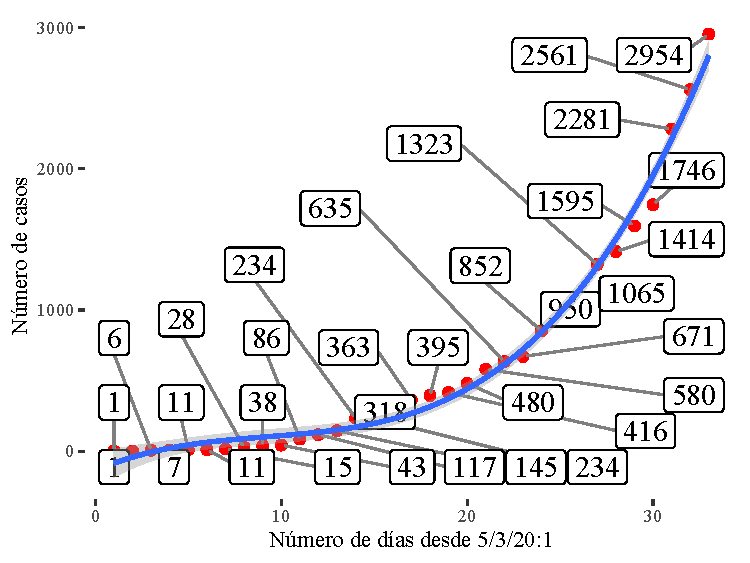
\includegraphics{E_1_files/figure-latex/ww1w-1} 

}

\caption{Regresión lineal}\label{fig:ww1w}
\end{figure}

\begin{verbatim}
## (Intercept) 
##    12917.13
\end{verbatim}

Sea la Tabla \ref{tab:2w3} Figures and tables with captions will be placed in \texttt{figure} and \texttt{table} environments, respectively.

\begin{longtable}[t]{cccccccccc}
\caption{\label{tab:2w3}Figures and tables with captions will be placed in `figure` }\\
\toprule
$Y_i$ & $f_i$ & $F_i$ & $F_i^*$ & $h_i$ & $H_i$ & $H_i^*$ & $h_i\%$ & $H_i\%$ & $H_i^*\%$\\
\midrule
ESTJ & 1 & 1 & 75 & 0.01 & 0.01 & 1.00 & 1.33 & 1.33 & 100.00\\
ESTJ & 2 & 3 & 150 & 0.03 & 0.04 & 2.00 & 2.67 & 4.00 & 200.00\\
ESTP & 3 & 6 & 150 & 0.04 & 0.08 & 2.00 & 4.00 & 8.00 & 200.00\\
ESFJ & 4 & 10 & 150 & 0.05 & 0.13 & 2.00 & 5.33 & 13.33 & 200.00\\
ESFP & 6 & 16 & 150 & 0.08 & 0.21 & 2.00 & 8.00 & 21.33 & 200.00\\
ISTJ & 6 & 22 & 155 & 0.08 & 0.29 & 2.07 & 8.00 & 29.33 & 206.67\\
ISTP & 7 & 29 & 157 & 0.09 & 0.39 & 2.09 & 9.33 & 38.67 & 209.33\\
ISFJ & 8 & 37 & 158 & 0.11 & 0.49 & 2.11 & 10.67 & 49.33 & 210.67\\
ISFP & 9 & 46 & 166 & 0.12 & 0.61 & 2.21 & 12.00 & 61.33 & 221.33\\
ENTJ & 10 & 56 & 166 & 0.13 & 0.75 & 2.21 & 13.33 & 74.67 & 221.33\\
ENTP & 6 & 62 & 166 & 0.08 & 0.83 & 2.21 & 8.00 & 82.67 & 221.33\\
ENFJ & 5 & 67 & 166 & 0.07 & 0.89 & 2.21 & 6.67 & 89.33 & 221.33\\
ENFP & 3 & 70 & 166 & 0.04 & 0.93 & 2.21 & 4.00 & 93.33 & 221.33\\
INTJ & 2 & 72 & 167 & 0.03 & 0.96 & 2.23 & 2.67 & 96.00 & 222.67\\
INTP & 1 & 73 & 169 & 0.01 & 0.97 & 2.25 & 1.33 & 97.33 & 225.33\\
INFJ & 1 & 74 & 172 & 0.01 & 0.99 & 2.29 & 1.33 & 98.67 & 229.33\\
INFP & 1 & 75 & 176 & 0.01 & 1.00 & 2.35 & 1.33 & 100.00 & 234.67\\
\bottomrule
\end{longtable}

  \bibliography{book.bib,packages.bib}

\printindex

\end{document}
